\documentclass[english, twocolumn]{article}
%%%%%%%%%%%%%%%%%%%%%%%%%%%%%%%%%%%%%%%%%%%%%%%%%%%%%%%%%%%%%%%%%%%%%%%%%%%%%%%%%%%%%%%%%%%%%%%%%%%%%%%%%%%%%%%%%%%%%%%%%%%%
\usepackage{latexsym,amsmath,amssymb,amsfonts,hyperref,fullpage,graphicx, float,adjustbox}
\usepackage{lastpage,listings}
\usepackage[hang, small,labelfont=bf,up,textfont=it,up]{caption} % Custom captions under/above floats in tables or figures
\usepackage{placeins}
\usepackage{adjustbox}
\usepackage[toc,page]{appendix}
\usepackage{tabulary}
\usepackage[margin=0.5in]{geometry}
\title{MEAM 620 Project 3} 
\author{Lou Lin, Mary Ibrahim, Gabrielle Merritt}
\begin{document}
\maketitle

\begin{abstract}
For this project we used an off the shelf commercial drone, and wrote custom software for it to run commanded closed loop trajectories. Leveraging our knowledge about quadrotor controllers and trajectory planning from the previous projects we were able to make our Bebop drone fly four different trajectories, and the potential to run any straight line trajectory. 
\end{abstract}
\section*{Code Architecture }
For the code architecture, we used the Bebop's SDK basic flying sample as a base to send and receive messages from the Bebop, and used it as a basis for designing our trajectory planning and control code. Using BebopDecodeStream as our basis, we added a trajectory planner, which reads trajectory coefficients and the time it takes to execute the segment  from a text file.After reading in the coefficients and segment time, we use the current time to calculate our desired position,velocity and acceleration, which we feed into our controller. Our controller uses the quads current orientation and velocity in order to estimate our current state and the desired state from the trajectory generator , and returns our commanded orientation and z velocity. Once the time for each segment is completed we read in a new set of trajectory coefficients and segment times, until we have finished reading the trajectory text file. Please refer to the figure below.
\begin{figure}[h!] 
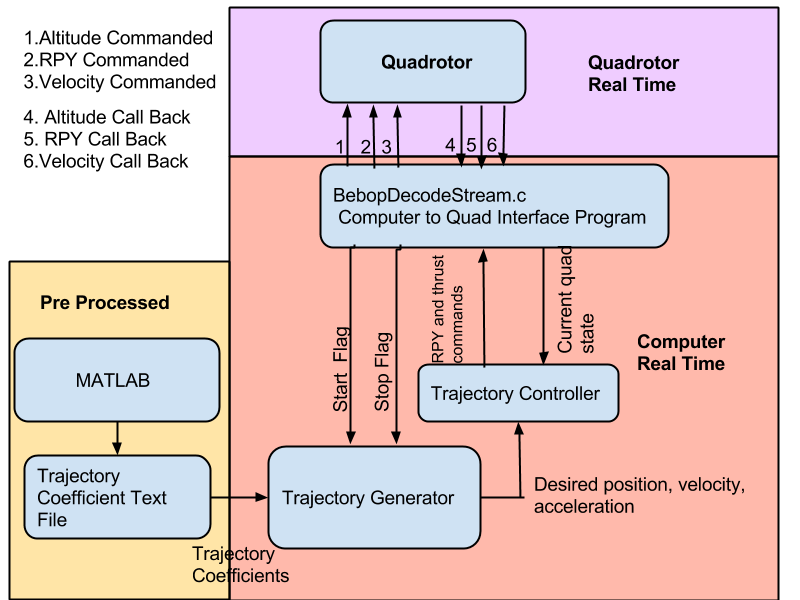
\includegraphics[width = \linewidth]{software.png}
\label{fig:code_draw}
\caption{Diagram of Code Architecture}
\end{figure}
\FloatBarrier 

\section*{Methods}
\subsection*{Control System}
\paragraph{Estimating Flight States}
To have the Bebop fly any arbitrary trajectory in $R^3$, a position based controller is necessary. In order to implement a position based controller, we must be able to estimate the position and orientation of the quadrotor. Since the video transferred through wifi is not reliable, using epipolar geometry related technique on the computer's side is impossible. Luckily, the Bebop drone already have onboard attitude and velocity estimator using a combination of inertial sensors and optical flow. Assuming the sensor fusion onboard is reliable, it is reasonable for me to just pull the information from the drone registering my own callback functions in the API. \\
 
 \begin{adjustbox}{width=.45*\textwidth, height=4*\textheight,keepaspectratio}
\begin{lstlisting}
ARCOMMANDS_Decoder_SetCommonCommonStateBatteryStateChangedCallback
(batteryStateChangedCallback, deviceManager);

ARCOMMANDS_Decoder_SetARDrone3PilotingStateFlyingStateChangedCallback
(flyingStateChangedCallback, deviceManager);

ARCOMMANDS_Decoder_SetARDrone3PilotingStateAltitudeChangedCallback
(altitudeCallback, deviceManager);

ARCOMMANDS_Decoder_SetARDrone3PilotingStateAttitudeChangedCallback
(attitudeCallback, deviceManager);

ARCOMMANDS_Decoder_SetARDrone3PilotingStateSpeedChangedCallback
(velocityCallback, deviceManager);
\end{lstlisting}
\end{adjustbox}
The velocity measured is already set in the world frame. Since the Bebop can directly measure altitude, all it's left to do is to numerically integrate the velocity in the x and y direction to obtain my position. We used forward Euler approximation to calculate our position, and the result were reasonable. \\

\paragraph{Actuator Inputs}
We are able to send 4 different inputs to the Bebop drone. The
\begin{verbatim}
ARCOMMANDS_Generator_GenerateARDrone3PilotingPCMD()
\end{verbatim} function 
allows me to send desired roll and pitch angles, the yaw rate, and the velocity
in the world Z direction. The inner loop from propeller inputs to the desired
roll, pitch, yaw and velocity in Z is already close onboard, and we have no 
access to it unless we hack the firmware, so we will just assume that the inner
loop is stable and reacts fast to the reference signals. It is interesting that the
API has two different definitions of the body frame. The reference frame for
the actuator inputs has a rotation of $\pi$ about the X axis of the sensor
reference frame, therefore the controller needs to be modified accordingly.\\

\paragraph{Backstepping Control of position}
Leveraging from project 1 phase 2, we can just take a controller in this form and expect the errors converge to zero exponentially.
$$a_{i commanded} = a_{i desired} + K_{di}(V_{i desired} - V_i) + K_{p i}(r_{i desired} - r_i)$$

Then we can linearize about hover and use the commanded acceleration in the X and Y direction to find the desired roll and pitch angles. As long as the onboard attitude controller make these angles converge to the desired values much faster than my position controller, the quadrotor will perform reasonably.\\

However, the reference frames are defined differently. In the sensor frame, the Z axis points down, and the Z axis points up. In order to compensate for this inconsistency, I have to negate the pitch angle and the desired velocity in the Z direction.
$$
\phi_{commanded} = g(a_{x commanded}*\sin\psi - a_{y commanded})\cos\psi
$$
$$\theta_{commanded} = -g(a_{x commanded}*\cos\psi + a_{y commanded})\sin\psi$$


Note that I can only command desired Z velocity instead of a thrust. I must modify the control law for the commanded Z velocity (such is named gaz in the API).
\begin{equation}
gaz = V_{z desired} + K_{pz}(r_{z desired} - r_z)
\end{equation}

\subsection*{Trajectory Generation}
We used MATLAB to generate coefficients for quintic minimum jerk trajectories. For trajectories composed of successive straight line segments, each line was planned over $10√((x_f-x_0 )^2+(y_f-y_0 )^2+(z_f-z_0 )^2 )$ seconds, with the quadrotor stopping at each waypoint.  We calculated coefficients$ a_0$,$a_1$,$a_2$,$a_3$,$a_4$ and $a_5$ in the x, y, and z directions based on the start and end positions of each line segment and start and end velocities and accelerations of zero. We then output the coefficients and length of time for each segment to a text file. After reading the text file into C, we calculated the time-parameterized position, velocity, and acceleration: 
$$x= a_0+ a_1 t+a_2 t^2+ a_3 t^3+ a_4 t^4+a_5 t^5$$
$$\dot{x}=a_1+2a_2 t+ 3a_3 t^2+ 4a_4 t^3+a5_5 t^4$$
$$\ddot{x}=2a_2+ 6a_3 t+ 12a_4 t^2+20a_5 t^3$$

These values were the desired positions, velocities, and accelerations that we fed into our controller. We used this method to generate a closed square trajectory. 

For curved trajectories, we used parametric equations for x and y and had the parameter θ vary according to a quintic. We created a figure 8 trajectory in the x-y plane with the position equations: 
$$x=r cos⁡θ-r$$
$$y=r sin⁡2θ$$
$$z=-1$$
Similarly, we created a circle trajectory with the equations:
$$x=r cos⁡θ-r$$
$$y=r sin⁡θ$$
$$z=-1
$$
In MATLAB, we calculated coefficients$ a_0$,$a_1$,$a_2$,$a_3$,$a_4$ and $a_5$for θ as it varies from zero to $2\pi$ and output these coefficients and the time to complete the entire trajectory to a text file. After reading these coefficients into C, we calculated θ,$\dot{θ}$,̇ and $\ddot{θ }$  and used these to calculate x and y positions, velocities, and accelerations, holding z constant. 



\subsubsection*{Curved trajectories}
For curved trajectories, we used parametric equations for x and y and had the parameter  vary according to a quintic. We created a figure 8 trajectory in the x-y plane with the position equations: 
 $$theta = a0 + a1*t +a2*t^2 + a3*t^3 + a4*t^4 + a5*t^5 
 $$
 $$ omega = a1 + 2*a2*t + 3*a3*t^2 + 4*a4*t^3 + 5*a5*t^4
 $$
 $$ alpha = 2*a2 + 6*a3*t + 12*a4*t^2 + 20*a5*t^3;
 $$
 $$x = r*cos(theta)-r $$
 $$ y = r*sin(n*theta)$$
 $$  z = -1 $$

In MATLAB, we calculated coefficients  and  for  as it varies from zero to  and output these coefficients and the time to complete the entire trajectory to a text file. After reading these coefficients into C, we calculated  and and used these to calculate x and y positions, velocities, and accelerations, holding z constant.
\section*{Results} 
\subsection*{Circle trajectory}
Our plots for our circle trajectory with a diameter of 1 meter. Our actual position tracks our desired position relatively well (See figure~\ref{fig:circle_3d}. Our quadrotor was able to maintain its hover position at our desired z height – the offset before and after the trajectory is due to our bookkeeping of height, and the spikes in z velocity correspond to takeoff and landing. Our x and y positions also track well but they lag somewhat and overshoot the desired position. This seems mostly due to the aggressive trajectory. With 12 seconds to complete the trajectory, the quadrotor wasn’t quite able to keep up with the desired position and velocity inputs. There may also have been issues resulting from the linear nature of our controller. A radius of .5 meters is tight relative to the size of the quadrotor, and requires roll and pitch angles that may be too large to adhere strictly to our assumption of linearity. Finally, the irregularities in our velocity feedback could have resulted from how the Bebop measures velocity. It uses optical flow to provide velocity feedback, and the surface of the floor during this test did not have an abundance of good features to aid in optical flow calculations. 

\subsection*{Demo Trajectories }
The figure 8 (Figure~\ref{fig:helix_square2} and square trajectories are the ones we ran during our demo. Figure 8 tracking suffered from a lot of the same issues as the circle – it was trying to follow an aggressive trajectory in a short amount of time (also 12 seconds) and couldn’t keep up. We see this especially in the y position and velocity graphs, where the figure 8 corresponds to the trajectory between 80 and 100 seconds. It also may have required roll and pitch angles that broke our assumption of linear dynamics. 

For the square part of the trajectory, the quadrotor's on board position tracking seems to have been miscalibrated. In Figure~\ref{fig:helix_square1} you can see the quadrotor start to veer severely to the right in the y direction, two fifths of the way through the trajectory, we believe this occured because the downward facing camera lost track of one of the April tags, and miscalculated its relative and position and velocity. 

\FloatBarrier
\section*{\\Graphs} \label{App:AppendixA}
All of the graphs below have negative values for Z position, this is because our reference frame has negative Z pointing upwards. 
\FloatBarrier
\begin{figure}[h!]
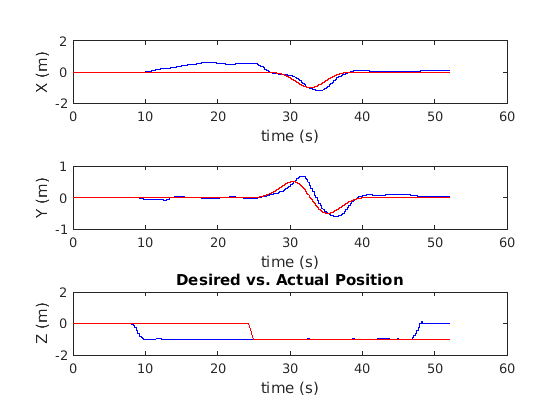
\includegraphics[width = \linewidth]{circle_pos.png}
\caption{Actual position versus Desired position}
\label{fig:circle_3d}
\end{figure}
\begin{figure}[h!]
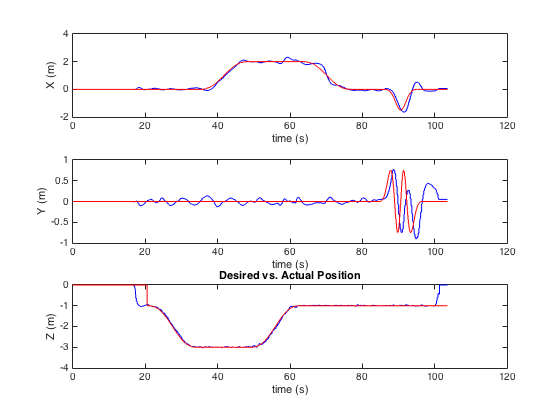
\includegraphics[width = \linewidth]{helix_square_pos.png}
\caption{Actual position versus Desired position for Helix and Square Trajectories (Z frame is flipped) }
\label{fig:helix_square}
\end{figure}
\begin{figure}[h!]
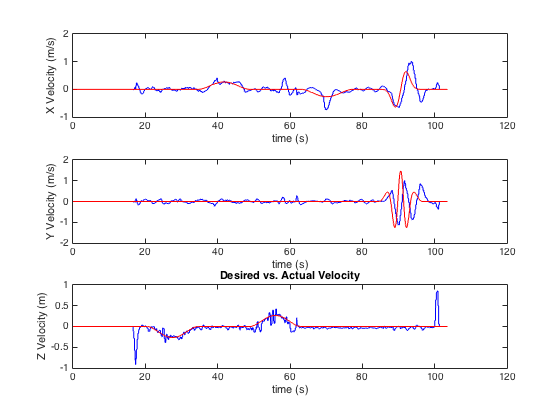
\includegraphics[width = \linewidth]{helix_square_vel.png}
\caption{Actual position versus Desired position for Helix and Square Trajectories}
\label{fig:helix_square1}
\end{figure}
\begin{figure}[h!]
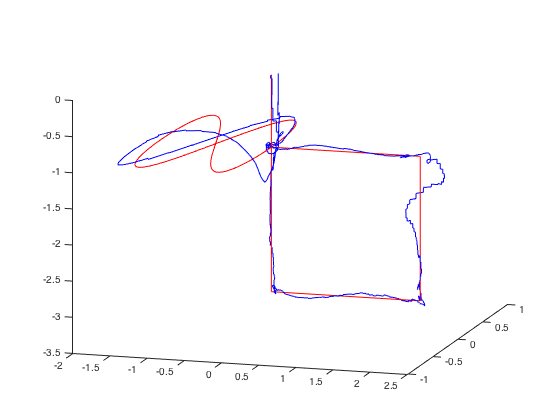
\includegraphics[width = \linewidth]{helix_square_3d.png}
\caption{Actual position versus Desired position for Helix and Square Trajectories}
\label{fig:helix_square2}
\end{figure}
\href{https://www.youtube.com/watch?v=sI6rJ2HQ4nc}{Link for Helix trajectory Video}
\\
\href{https://www.youtube.com/watch?v=-9Lq45Qe26Q}{Link forSquare Trajectory Video}

\end{document}
